\documentclass[10pt]{beamer}

% Packages
\usepackage[utf8]{inputenc}
\usepackage[T1]{fontenc}
\usepackage{amsmath, amssymb, amsthm}
\usepackage{graphicx}
\usepackage{booktabs}
\usepackage{hyperref}
\usepackage{tikz}
\usetikzlibrary{trees, positioning, shapes, arrows.meta, patterns, decorations.pathreplacing, calc}

\usepackage{algorithm}
\usepackage{algpseudocode}

% Theme settings
\usetheme{default}
\usecolortheme{default}
\usefonttheme{professionalfonts}

% Color definitions (minimalist academic palette)
\definecolor{ThemeBlue}{RGB}{0, 62, 116}
\definecolor{DarkGray}{RGB}{51, 51, 51}
\definecolor{LightGray}{RGB}{245, 245, 245}
\definecolor{AccentOrange}{RGB}{214, 96, 77}
\definecolor{AccentGreen}{RGB}{0, 128, 0}
\definecolor{LightBlue}{RGB}{200, 220, 240}
\definecolor{LightOrange}{RGB}{255, 220, 200}
\definecolor{LightGreen}{RGB}{200, 240, 200}

% Apply colors
\setbeamercolor{frametitle}{fg=ThemeBlue, bg=white}
\setbeamercolor{title}{fg=ThemeBlue}
\setbeamercolor{structure}{fg=ThemeBlue}
\setbeamercolor{normal text}{fg=DarkGray}
\setbeamercolor{block title}{fg=white, bg=ThemeBlue}
\setbeamercolor{block body}{fg=DarkGray, bg=LightGray}
\setbeamercolor{itemize item}{fg=ThemeBlue}
\setbeamercolor{enumerate item}{fg=ThemeBlue}

% Remove navigation symbols
\setbeamertemplate{navigation symbols}{}

% Customize frame title
\setbeamertemplate{frametitle}{
  \vspace{0.5em}
  \insertframetitle
  \vspace{0.3em}
}

% Customize itemize
\setbeamertemplate{itemize items}[circle]
\setlength{\leftmargini}{1.5em}

% Footer
\setbeamertemplate{footline}{
  \leavevmode%
  \hbox{%
  \begin{beamercolorbox}[wd=.333333\paperwidth,ht=2.25ex,dp=1ex,left]{author in head/foot}%
    \hspace{1em}\usebeamerfont{author in head/foot}\insertshortauthor
  \end{beamercolorbox}%
  \begin{beamercolorbox}[wd=.333333\paperwidth,ht=2.25ex,dp=1ex,center]{title in head/foot}%
    \usebeamerfont{title in head/foot}\insertshorttitle
  \end{beamercolorbox}%
  \begin{beamercolorbox}[wd=.333333\paperwidth,ht=2.25ex,dp=1ex,right]{date in head/foot}%
    \usebeamerfont{date in head/foot}\insertshortdate{}\hspace*{2em}
    \insertframenumber{} / \inserttotalframenumber\hspace*{2ex}
  \end{beamercolorbox}}%
  \vskip0pt%
}

% Title page customization
\setbeamertemplate{title page}{
  \vbox{}
  \vfill
  \begingroup
    \centering
    {\usebeamercolor[fg]{title}\usebeamerfont{title}\inserttitle\par}
    \vskip0.5em
    {\usebeamercolor[fg]{subtitle}\usebeamerfont{subtitle}\insertsubtitle\par}
    \vskip2em
    {\usebeamercolor[fg]{author}\usebeamerfont{author}\insertauthor\par}
    \vskip0.5em
    {\usebeamercolor[fg]{institute}\usebeamerfont{institute}\insertinstitute\par}
    \vskip1em
    {\usebeamercolor[fg]{date}\usebeamerfont{date}\insertdate\par}
  \endgroup
  \vfill
}

% Commands for highlighting
\newcommand{\highlight}[1]{\textcolor{AccentOrange}{\textbf{#1}}}
\newcommand{\emphbox}[1]{\colorbox{LightGray}{\textcolor{DarkGray}{#1}}}

% Mathematical operators
\DeclareMathOperator*{\argmin}{arg\,min}
\DeclareMathOperator*{\argmax}{arg\,max}
\DeclareMathOperator{\E}{\mathbb{E}}
\DeclareMathOperator{\Var}{Var}
\DeclareMathOperator{\Cov}{Cov}
\DeclareMathOperator{\Corr}{Corr}
\DeclareMathOperator{\MSE}{MSE}
\DeclareMathOperator{\RSS}{RSS}
\DeclareMathOperator{\sign}{sign}

%----------------------------------------------------------------------------------------
% TITLE PAGE
%----------------------------------------------------------------------------------------

\title{Big Data in Finance}
\subtitle{Week 7: Neural Networks}
\author{Dr Daniele Bianchi}
\date{Spring 2026}

%----------------------------------------------------------------------------------------
% DOCUMENT
%----------------------------------------------------------------------------------------

\begin{document}

\AtBeginSection[]{
  \begin{frame}[plain]
    \vfill
    \begin{center}
      {\Large\color{ThemeBlue}\insertsection}
    \end{center}
    \vfill
  \end{frame}
}


% Title slide
\begin{frame}[plain]
  \titlepage
\end{frame}

% Outline slide
\begin{frame}{Today's Agenda}
  \tableofcontents
\end{frame}

%----------------------------------------------------------------------------------------
\section{From What We Know to Neural Networks}
%----------------------------------------------------------------------------------------

\begin{frame}{Recap: Our Toolkit So Far}

  \textbf{We've learned several approaches to prediction:}

  \vspace{1em}
  \begin{itemize}
    \item \textbf{Linear methods} (Week 2): Ridge, Lasso, Elastic Net
    \begin{itemize}
      \item Global model: same coefficients everywhere
      \item Smooth predictions, easy to interpret
    \end{itemize}

    \vspace{0.5em}
    \item \textbf{Tree-based methods} (Week 3): Random Forests, XGBoost
    \begin{itemize}
      \item Local models: different rules in different regions
      \item Capture interactions automatically
    \end{itemize}

    \vspace{0.5em}
    \item \textbf{Classification} (Week 4): Logistic regression, tree ensembles
    \begin{itemize}
      \item Predicting probabilities (e.g., default risk)
      \item The sigmoid function ``squashes'' outputs to $[0, 1]$
    \end{itemize}
  \end{itemize}

  \vspace{0.5em}
  \begin{block}{Today's Question}
    Is there a method that combines the best of both worlds?
  \end{block}
\end{frame}

%----------------------------------------------------------------------------------------

\begin{frame}{The Gap We Want to Fill}

  \begin{center}
  \begin{tabular}{lcc}
    \toprule
    & \textbf{Linear Models} & \textbf{Trees} \\
    \midrule
    Smooth predictions & \textcolor{AccentGreen}{\checkmark} & \textcolor{AccentOrange}{$\times$} \\
    Captures non-linearity & \textcolor{AccentOrange}{$\times$} & \textcolor{AccentGreen}{\checkmark} \\
    Finds interactions automatically & \textcolor{AccentOrange}{$\times$} & \textcolor{AccentGreen}{\checkmark} \\
    Works well with many features & \textcolor{AccentGreen}{\checkmark} (with regularization) & \textcolor{AccentGreen}{\checkmark} \\
    Extrapolates beyond training data & \textcolor{AccentGreen}{\checkmark} & \textcolor{AccentOrange}{$\times$} \\
    \bottomrule
  \end{tabular}
  \end{center}

  \vspace{1em}
  \textbf{What if we want:}
  \begin{itemize}
    \item Smooth predictions (like linear models)
    \item But also captures complex non-linear patterns (like trees)
    \item And learns which interactions matter from the data
  \end{itemize}

  \vspace{0.5em}
  \highlight{Neural networks} offer this flexibility---but with trade-offs we'll discuss.
\end{frame}

%----------------------------------------------------------------------------------------

\begin{frame}{A Financial Motivation}

  \textbf{Return prediction:} Complex patterns that simple models might miss

  \vspace{0.5em}
  \begin{itemize}
    \item \textbf{Non-linear effects:} Dividend yield might predict returns differently at extreme values vs.\ normal values

    \vspace{0.3em}
    \item \textbf{Interactions:} The effect of valuation ratios might depend on the level of interest rates

    \vspace{0.3em}
    \item \textbf{Regime dependence:} Predictability might differ in recessions vs.\ expansions
  \end{itemize}

  \vspace{1em}
  \textbf{Credit risk:} Complex borrower profiles
  \begin{itemize}
    \item Default risk depends on combinations of factors
    \item A borrower with high income \textit{and} high debt is different from one with high income \textit{and} low debt
    \item Trees capture this, but predictions are ``blocky''
  \end{itemize}

  \vspace{0.5em}
  \begin{block}{The Promise}
    Neural networks can learn \highlight{smooth, non-linear functions} from data
  \end{block}
\end{frame}

%----------------------------------------------------------------------------------------
\section{The Single Neuron: Building Block}
%----------------------------------------------------------------------------------------

\begin{frame}{You Already Know This! (Almost)}

  \textbf{Recall logistic regression from Week 4:}
  \[
  P(\text{default}) = \sigma\left(\beta_0 + \beta_1 x_1 + \beta_2 x_2 + \cdots\right)
  \]

  where $\sigma(z) = \frac{1}{1 + e^{-z}}$ is the \highlight{sigmoid function}

  \vspace{1em}
  \textbf{What logistic regression does:}
  \begin{enumerate}
    \item Take a \textbf{weighted sum} of inputs: $z = \beta_0 + \beta_1 x_1 + \cdots$
    \item Pass it through a \textbf{non-linear function} (sigmoid)
    \item Output a value between 0 and 1
  \end{enumerate}

  \vspace{1em}
  \begin{block}{Key Insight}
    A single \highlight{neuron} does exactly this! Logistic regression \textit{is} a one-neuron neural network.
  \end{block}
\end{frame}

%----------------------------------------------------------------------------------------

\begin{frame}{The Single Neuron}

  \begin{center}
  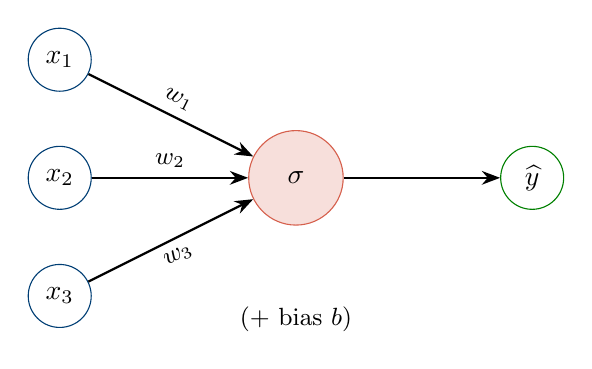
\begin{tikzpicture}[
    node distance=1.5cm,
    input/.style={circle, draw=ThemeBlue, minimum size=0.8cm},
    neuron/.style={circle, draw=AccentOrange, fill=AccentOrange!20, minimum size=1.2cm},
    output/.style={circle, draw=AccentGreen, minimum size=0.8cm},
    arrow/.style={-{Stealth}, thick}
  ]
    % Inputs
    \node[input] (x1) at (0, 1.5) {$x_1$};
    \node[input] (x2) at (0, 0) {$x_2$};
    \node[input] (x3) at (0, -1.5) {$x_3$};

    % Neuron
    \node[neuron] (n) at (3, 0) {$\sigma$};

    % Output
    \node[output] (y) at (6, 0) {$\widehat{y}$};

    % Arrows with weights
    \draw[arrow] (x1) -- node[above, sloped] {\small $w_1$} (n);
    \draw[arrow] (x2) -- node[above] {\small $w_2$} (n);
    \draw[arrow] (x3) -- node[below, sloped] {\small $w_3$} (n);
    \draw[arrow] (n) -- (y);

    % Bias
    \node at (3, -1.8) {\small (+ bias $b$)};
  \end{tikzpicture}
  \end{center}

  \vspace{0.5em}
  \textbf{A neuron computes:}
  \[
  \widehat{y} = \sigma\underbrace{(w_1 x_1 + w_2 x_2 + w_3 x_3 + b)}_{\text{weighted sum + bias}}
  \]

  \vspace{0.5em}
  \begin{itemize}
    \item \textbf{Weights} ($w_1, w_2, w_3$): How much each input matters (like $\beta$ coefficients)
    \item \textbf{Bias} ($b$): Shifts the decision threshold (like intercept $\beta_0$)
    \item \textbf{Activation function} ($\sigma$): Introduces non-linearity
  \end{itemize}
\end{frame}

%----------------------------------------------------------------------------------------

\begin{frame}{Why Do We Need the Non-Linear Function?}

  \textbf{Without the activation function:}
  \[
  \text{Neuron output} = w_1 x_1 + w_2 x_2 + \cdots + b
  \]
  This is just linear regression!

  \vspace{1em}
  \textbf{The problem:} Stacking linear functions gives... another linear function
  \[
  f(g(x)) = f(ax + b) = c(ax + b) + d = (ca)x + (cb + d)
  \]
  Still linear! No matter how many layers, you get a linear model.

  \vspace{1em}
  \textbf{The solution:} Non-linear activation functions ``break'' the linearity
  \begin{itemize}
    \item Allow the network to learn curved decision boundaries
    \item Enable approximation of complex functions
  \end{itemize}

  \vspace{0.5em}
  \begin{block}{Key Point}
    The activation function is what makes neural networks powerful. Without it, we'd just have a fancy linear regression.
  \end{block}
\end{frame}

%----------------------------------------------------------------------------------------

\begin{frame}{Common Activation Functions}

  \begin{center}
  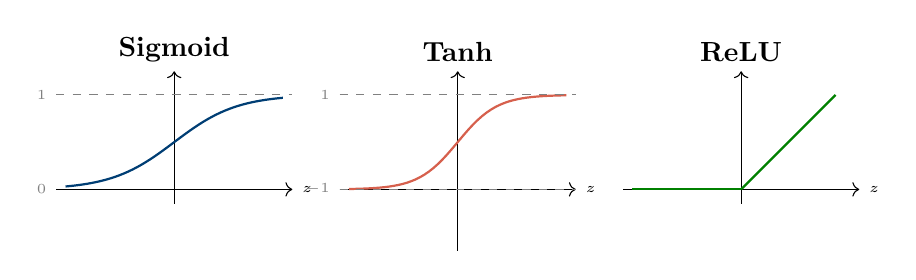
\begin{tikzpicture}[scale=0.6]
    % Sigmoid
    \begin{scope}[shift={(0,0)}]
      \draw[->] (-2.5,0) -- (2.5,0) node[right] {\tiny $z$};
      \draw[->] (0,-0.3) -- (0,2.5);
      \draw[thick, ThemeBlue, domain=-2.3:2.3, samples=50] plot (\x, {2/(1+exp(-1.5*\x))});
      \node[above] at (0,2.5) {\textbf{Sigmoid}};
      \draw[dashed, gray] (-2.5,2) -- (2.5,2);
      \node[left, gray, font=\tiny] at (-2.5,2) {1};
      \node[left, gray, font=\tiny] at (-2.5,0) {0};
    \end{scope}

    % tanh
    \begin{scope}[shift={(6,0)}]
      \draw[->] (-2.5,0) -- (2.5,0) node[right] {\tiny $z$};
      \draw[->] (0,-1.3) -- (0,2.5);
      \draw[thick, AccentOrange, domain=-2.3:2.3, samples=50] plot (\x, {tanh(1.2*\x) + 1});
      \node[above] at (0,2.5) {\textbf{Tanh}};
      \draw[dashed, gray] (-2.5,2) -- (2.5,2);
      \draw[dashed, gray] (-2.5,0) -- (2.5,0);
      \node[left, gray, font=\tiny] at (-2.5,2) {1};
      \node[left, gray, font=\tiny] at (-2.5,0) {$-$1};
    \end{scope}

    % ReLU
    \begin{scope}[shift={(12,0)}]
      \draw[->] (-2.5,0) -- (2.5,0) node[right] {\tiny $z$};
      \draw[->] (0,-0.3) -- (0,2.5);
      \draw[thick, AccentGreen, domain=-2.3:0] plot (\x, 0);
      \draw[thick, AccentGreen, domain=0:2] plot (\x, \x);
      \node[above] at (0,2.5) {\textbf{ReLU}};
    \end{scope}
  \end{tikzpicture}
  \end{center}

  \begin{center}
  \begin{tabular}{lcl}
    \toprule
    \textbf{Function} & \textbf{Formula} & \textbf{Notes} \\
    \midrule
    Sigmoid & $\frac{1}{1+e^{-z}}$ & Output in $(0, 1)$; used in logistic regression \\[0.3em]
    Tanh & $\frac{e^z - e^{-z}}{e^z + e^{-z}}$ & Output in $(-1, 1)$; centered around 0 \\[0.3em]
    ReLU & $\max(0, z)$ & Modern default; simple and effective \\
    \bottomrule
  \end{tabular}
  \end{center}

  \vspace{0.5em}
  \textbf{For this course:} We'll primarily use \highlight{ReLU} (Rectified Linear Unit)---it's the most common choice in practice.
\end{frame}

%----------------------------------------------------------------------------------------

\begin{frame}{ReLU: The Workhorse of Modern Neural Networks}

  \textbf{ReLU is surprisingly simple:}
  \[
  \text{ReLU}(z) = \max(0, z) = \begin{cases} z & \text{if } z > 0 \\ 0 & \text{if } z \leq 0 \end{cases}
  \]

  \vspace{0.5em}
  \textbf{Why is this so popular?}
  \begin{itemize}
    \item \textit{Computationally simple:} Just check if input is positive
    \item \textit{Avoids ``vanishing gradients'':} A technical problem we'll mention later
    \item \textit{Sparsity:} Many neurons output zero, making networks efficient
  \end{itemize}

  \vspace{1em}
  \textbf{Intuition:} ReLU acts like a ``gate''
  \begin{itemize}
    \item If the weighted input is positive: pass it through
    \item If the weighted input is negative: block it (output zero)
  \end{itemize}

  \vspace{0.5em}
  This allows the network to ``turn on'' different neurons for different inputs, creating complex patterns.
\end{frame}

%----------------------------------------------------------------------------------------
\section{Building a Network: Multiple Neurons}
%----------------------------------------------------------------------------------------

\begin{frame}{One Neuron Isn't Enough}

  \textbf{A single neuron with sigmoid = logistic regression}
  \begin{itemize}
    \item Can only learn linear decision boundaries
    \item Limited expressive power
  \end{itemize}

  \vspace{1em}
  \textbf{The solution: Combine multiple neurons}

  \begin{center}
  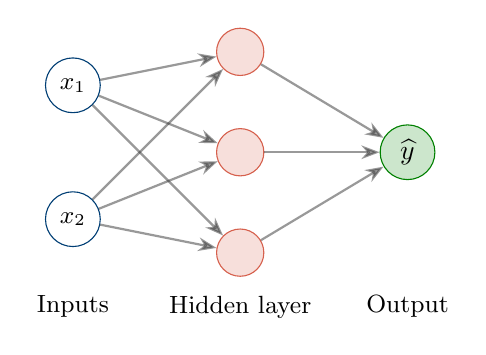
\begin{tikzpicture}[
    scale=0.85,
    node distance=1.2cm,
    input/.style={circle, draw=ThemeBlue, minimum size=0.6cm, font=\small},
    neuron/.style={circle, draw=AccentOrange, fill=AccentOrange!20, minimum size=0.6cm},
    output/.style={circle, draw=AccentGreen, fill=AccentGreen!20, minimum size=0.6cm},
    arrow/.style={-{Stealth}, thick, DarkGray}
  ]
    % Inputs
    \node[input] (x1) at (0, 1) {$x_1$};
    \node[input] (x2) at (0, -1) {$x_2$};

    % Hidden neurons
    \node[neuron] (h1) at (2.5, 1.5) {};
    \node[neuron] (h2) at (2.5, 0) {};
    \node[neuron] (h3) at (2.5, -1.5) {};

    % Output
    \node[output] (y) at (5, 0) {$\widehat{y}$};

    % Connections: input to hidden
    \foreach \i in {1,2} {
      \foreach \j in {1,2,3} {
        \draw[arrow, opacity=0.5] (x\i) -- (h\j);
      }
    }

    % Connections: hidden to output
    \foreach \j in {1,2,3} {
      \draw[arrow, opacity=0.5] (h\j) -- (y);
    }

    % Labels
    \node[below] at (0, -2) {\small Inputs};
    \node[below] at (2.5, -2) {\small Hidden layer};
    \node[below] at (5, -2) {\small Output};
  \end{tikzpicture}
  \end{center}

  \vspace{0.3em}
  Each hidden neuron learns to detect a different pattern in the data.
\end{frame}

%----------------------------------------------------------------------------------------

\begin{frame}{The Multi-Layer Perceptron (MLP)}

  \textbf{Architecture:} Stack neurons into layers

  \begin{center}
  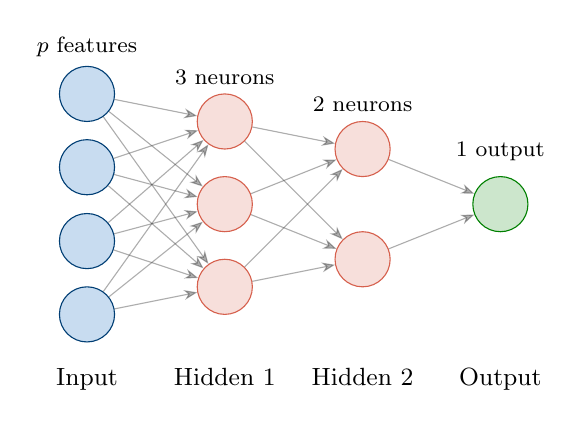
\begin{tikzpicture}[
    scale=0.7,
    node distance=1cm,
    input/.style={circle, draw=ThemeBlue, fill=LightBlue, minimum size=0.7cm, font=\small},
    hidden/.style={circle, draw=AccentOrange, fill=AccentOrange!20, minimum size=0.7cm},
    output/.style={circle, draw=AccentGreen, fill=AccentGreen!20, minimum size=0.7cm},
    arrow/.style={-{Stealth}, DarkGray, opacity=0.4}
  ]
    % Input layer
    \foreach \i/\y in {1/2, 2/0.67, 3/-0.67, 4/-2} {
      \node[input] (x\i) at (0, \y) {};
    }

    % Hidden layer 1
    \foreach \i/\y in {1/1.5, 2/0, 3/-1.5} {
      \node[hidden] (h1\i) at (2.5, \y) {};
    }

    % Hidden layer 2
    \foreach \i/\y in {1/1, 2/-1} {
      \node[hidden] (h2\i) at (5, \y) {};
    }

    % Output layer
    \node[output] (y) at (7.5, 0) {};

    % Connections
    \foreach \i in {1,...,4} {
      \foreach \j in {1,2,3} {
        \draw[arrow] (x\i) -- (h1\j);
      }
    }
    \foreach \i in {1,2,3} {
      \foreach \j in {1,2} {
        \draw[arrow] (h1\i) -- (h2\j);
      }
    }
    \foreach \i in {1,2} {
      \draw[arrow] (h2\i) -- (y);
    }

    % Labels
    \node[below] at (0, -2.8) {\small Input};
    \node[below] at (2.5, -2.8) {\small Hidden 1};
    \node[below] at (5, -2.8) {\small Hidden 2};
    \node[below] at (7.5, -2.8) {\small Output};

    % Layer sizes
    \node[above, font=\footnotesize] at (0, 2.5) {$p$ features};
    \node[above, font=\footnotesize] at (2.5, 2) {3 neurons};
    \node[above, font=\footnotesize] at (5, 1.5) {2 neurons};
    \node[above, font=\footnotesize] at (7.5, 0.6) {1 output};
  \end{tikzpicture}
  \end{center}

  \vspace{0.3em}
  \textbf{Terminology:}
  \begin{itemize}
    \item \textit{Input layer:} Your features ($x_1, \ldots, x_p$)
    \item \textit{Hidden layers:} Where the ``learning'' happens
    \item \textit{Output layer:} The prediction
    \item \textit{Fully connected:} Neurons between layers are all connected
  \end{itemize}
\end{frame}

%----------------------------------------------------------------------------------------

\begin{frame}{How Information Flows (Forward Propagation)}

  \textbf{Example:} A network with one hidden layer of 3 neurons

  \vspace{0.5em}
  \textbf{Step 1: Input to hidden layer}
  \begin{align*}
  h_1 &= \text{ReLU}(w_{11}x_1 + w_{12}x_2 + b_1) \\
  h_2 &= \text{ReLU}(w_{21}x_1 + w_{22}x_2 + b_2) \\
  h_3 &= \text{ReLU}(w_{31}x_1 + w_{32}x_2 + b_3)
  \end{align*}

  \textbf{Step 2: Hidden layer to output}
  \[
  \widehat{y} = v_1 h_1 + v_2 h_2 + v_3 h_3 + c
  \]

  \vspace{0.5em}
  \textbf{What's happening:}
  \begin{itemize}
    \item Each hidden neuron computes a \highlight{different combination} of inputs
    \item The output combines these learned ``features''
    \item The network learns \textit{what} combinations are useful
  \end{itemize}
\end{frame}

%----------------------------------------------------------------------------------------

\begin{frame}{An Economic Intuition}

  \textbf{Think of hidden neurons as ``derived features'':}

  \vspace{1em}
  \begin{columns}[T]
    \column{0.45\textwidth}
    \textbf{Credit risk example:}
    \begin{itemize}
      \item Input: income, debt, credit score
      \item Hidden neuron 1 might learn: ``debt-to-income stress''
      \item Hidden neuron 2 might learn: ``credit utilization pattern''
      \item Hidden neuron 3 might learn: ``income stability indicator''
    \end{itemize}

    \column{0.50\textwidth}
    \textbf{Return prediction example:}
    \begin{itemize}
      \item Input: D/P, term spread, inflation
      \item Hidden neuron 1 might learn: ``valuation regime''
      \item Hidden neuron 2 might learn: ``monetary policy stance''
      \item Hidden neuron 3 might learn: ``risk appetite indicator''
    \end{itemize}
  \end{columns}

  \vspace{1em}
  \begin{block}{Key Insight}
    The network \highlight{automatically} constructs useful features from raw inputs. You don't have to manually engineer interaction terms or non-linear transformations.
  \end{block}
\end{frame}

%----------------------------------------------------------------------------------------

\begin{frame}{Why Depth Matters}

  \textbf{Adding more layers allows more complex functions:}

  \vspace{0.5em}
  \begin{itemize}
    \item \textbf{1 hidden layer:} Can approximate any continuous function (in theory)
    \item \textbf{More layers:} Can represent the same function more \highlight{efficiently}
  \end{itemize}

  \vspace{1em}
  \textbf{Intuition:} Hierarchical feature learning
  \begin{itemize}
    \item Layer 1: Learn simple patterns (e.g., ``is debt-to-income high?'')
    \item Layer 2: Combine simple patterns (e.g., ``high DTI \textit{and} low income'')
    \item Layer 3: Even more complex combinations
  \end{itemize}

  \vspace{1em}
  \textbf{But for financial data:}
  \begin{itemize}
    \item We typically have limited observations (decades, not millions)
    \item Very deep networks can overfit badly
    \item \highlight{1--2 hidden layers} often sufficient
  \end{itemize}

  \vspace{0.3em}
  \textit{More is not always better!}
\end{frame}

%----------------------------------------------------------------------------------------

\begin{frame}{The Universal Approximation Theorem}

  \textbf{A remarkable theoretical result:}

  \vspace{1em}
  \begin{block}{Universal Approximation (informal)}
    A neural network with a \textit{single} hidden layer containing enough neurons can approximate \textit{any} continuous function to arbitrary accuracy.
  \end{block}

  \vspace{1em}
  \textbf{What this means:}
  \begin{itemize}
    \item Neural networks are extremely flexible
    \item In principle, they can learn any pattern in the data
  \end{itemize}

  \vspace{1em}
  \textbf{What this does NOT mean:}
  \begin{itemize}
    \item We can \textit{find} the right weights (optimization is hard)
    \item We have \textit{enough data} to learn the true function
    \item The network will \textit{generalize} well to new data
  \end{itemize}

  \vspace{0.5em}
  \highlight{``Can approximate''} $\neq$ \highlight{``Will approximate well in practice''}
\end{frame}

%----------------------------------------------------------------------------------------
\section{How Neural Networks Learn}
%----------------------------------------------------------------------------------------

\begin{frame}{The Learning Problem}

  \textbf{We have many parameters to learn:}
  \begin{itemize}
    \item Weights connecting every neuron to the next layer
    \item Biases for each neuron
  \end{itemize}

  \vspace{0.5em}
  \textbf{Example:} Network with 10 inputs, one hidden layer of 50 neurons, 1 output
  \begin{itemize}
    \item Input to hidden: $10 \times 50 = 500$ weights + $50$ biases
    \item Hidden to output: $50 \times 1 = 50$ weights + $1$ bias
    \item \textbf{Total: 601 parameters}
  \end{itemize}

  \vspace{1em}
  \textbf{The goal:} Find values for all these parameters that minimize prediction error

  \vspace{0.5em}
  \textbf{Just like before, we minimize a loss function:}
  \begin{itemize}
    \item Regression: Mean Squared Error (MSE)
    \item Classification: Cross-entropy (related to log-likelihood in logistic regression)
  \end{itemize}
\end{frame}

%----------------------------------------------------------------------------------------

\begin{frame}{No Closed-Form Solution}

  \textbf{Unlike Ridge regression}, we can't just solve an equation

  \vspace{1em}
  \begin{center}
  \begin{tabular}{ll}
    \toprule
    \textbf{Ridge} & \textbf{Neural Network} \\
    \midrule
    Linear in parameters & Non-linear in parameters \\
    Closed-form: $(X'X + \lambda I)^{-1}X'y$ & No closed-form solution \\
    One global optimum & Many local optima \\
    \bottomrule
  \end{tabular}
  \end{center}

  \vspace{1em}
  \textbf{The solution: Iterative optimization}
  \begin{enumerate}
    \item Start with random initial weights
    \item Compute predictions and errors
    \item Adjust weights to reduce error
    \item Repeat until convergence
  \end{enumerate}

  \vspace{0.5em}
  This is called \highlight{gradient descent}.
\end{frame}

%----------------------------------------------------------------------------------------

\begin{frame}{Gradient Descent: The Intuition}

  \textbf{Imagine you're lost in mountains at night and want to reach the lowest point:}

  \vspace{0.5em}
  \begin{enumerate}
    \item Feel the slope of the ground beneath your feet
    \item Take a step in the downhill direction
    \item Repeat
  \end{enumerate}

  \vspace{1em}
  \begin{center}
  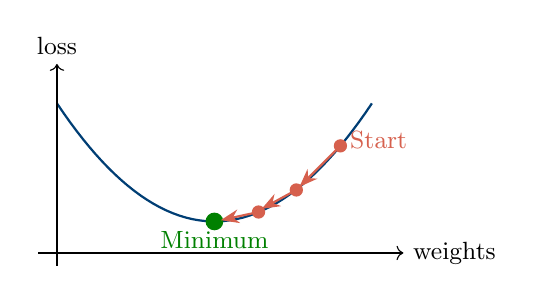
\begin{tikzpicture}[scale=0.8]
    % Loss surface
    \draw[thick, ThemeBlue, domain=0:5, samples=50] plot (\x, {0.3*(\x-2.5)^2 + 0.5});

    % Axes
    \draw[->] (-0.3, 0) -- (5.5, 0) node[right] {\small weights};
    \draw[->] (0, -0.2) -- (0, 3) node[above] {\small loss};

    % Gradient descent steps
    \fill[AccentOrange] (4.5, 1.7) circle (3pt);
    \fill[AccentOrange] (3.8, 1.0) circle (3pt);
    \fill[AccentOrange] (3.2, 0.65) circle (3pt);
    \fill[AccentGreen] (2.5, 0.5) circle (4pt);

    \draw[-{Stealth}, AccentOrange, thick] (4.5, 1.7) -- (3.85, 1.05);
    \draw[-{Stealth}, AccentOrange, thick] (3.8, 1.0) -- (3.25, 0.7);
    \draw[-{Stealth}, AccentOrange, thick] (3.2, 0.65) -- (2.6, 0.52);

    % Labels
    \node[above right, AccentOrange] at (4.5, 1.5) {\small Start};
    \node[below, AccentGreen] at (2.5, 0.5) {\small Minimum};
  \end{tikzpicture}
  \end{center}

  \vspace{0.3em}
  \textbf{Gradient descent:} ``Gradient'' = slope; ``Descent'' = go downhill
\end{frame}

%----------------------------------------------------------------------------------------

\begin{frame}{The Gradient Descent Update Rule}

  \textbf{At each step, update each weight:}
  \[
  w^{\text{new}} = w^{\text{old}} - \eta \cdot \frac{\partial \text{Loss}}{\partial w}
  \]

  \vspace{0.5em}
  \textbf{Components:}
  \begin{itemize}
    \item $\frac{\partial \text{Loss}}{\partial w}$: The gradient (slope) --- tells us which direction is ``downhill''
    \item $\eta$: The \highlight{learning rate} --- how big a step to take
    \item Minus sign: We want to go \textit{down}hill
  \end{itemize}

  \vspace{1em}
  \textbf{The learning rate is crucial:}
  \begin{itemize}
    \item Too large: Overshoot the minimum, might never converge
    \item Too small: Takes forever to converge
    \item Just right: Converges smoothly to a good solution
  \end{itemize}

  \vspace{0.3em}
  \textit{We'll see how to choose this in sklearn next week.}
\end{frame}

%----------------------------------------------------------------------------------------

\begin{frame}{Backpropagation: Computing the Gradients}

  \textbf{The challenge:} How do we compute $\frac{\partial \text{Loss}}{\partial w}$ for all weights?

  \vspace{1em}
  \textbf{The answer: Backpropagation} (short for ``backward propagation of errors'')

  \vspace{0.5em}
  \begin{enumerate}
    \item \textbf{Forward pass:} Compute predictions by passing inputs through the network
    \item \textbf{Compute loss:} Compare predictions to true values
    \item \textbf{Backward pass:} Use the chain rule to compute how each weight contributed to the error
  \end{enumerate}

  \vspace{1em}
  \begin{block}{Good News}
    You don't need to implement this! sklearn (and all neural network libraries) compute gradients automatically. Just understand the intuition.
  \end{block}

  \vspace{0.5em}
  \textbf{Intuition:} Errors at the output ``propagate back'' through the network, telling each weight how much it contributed to the mistake.
\end{frame}

%----------------------------------------------------------------------------------------

\begin{frame}{Stochastic Gradient Descent (SGD)}

  \textbf{Problem:} Computing gradients over the entire dataset is slow

  \vspace{0.5em}
  \textbf{Solution:} Use a random subset (``mini-batch'') at each step

  \vspace{1em}
  \begin{center}
  \begin{tabular}{lp{7cm}}
    \toprule
    \textbf{Method} & \textbf{Description} \\
    \midrule
    Batch GD & Use all data points for each update (slow but stable) \\
    Stochastic GD & Use one random point per update (fast but noisy) \\
    Mini-batch GD & Use a small batch (e.g., 32 points) --- best of both worlds \\
    \bottomrule
  \end{tabular}
  \end{center}

  \vspace{1em}
  \textbf{Why mini-batches work:}
  \begin{itemize}
    \item Approximate the true gradient well enough
    \item Much faster per iteration
    \item Some noise can actually help escape local minima
  \end{itemize}

  \vspace{0.5em}
  \textit{sklearn's default solver (``adam'') uses an advanced version of SGD.}
\end{frame}

%----------------------------------------------------------------------------------------

\begin{frame}{Modern Optimizers: Adam}

  \textbf{Plain gradient descent has limitations:}
  \begin{itemize}
    \item Same learning rate for all parameters
    \item Can get stuck or oscillate
  \end{itemize}

  \vspace{1em}
  \textbf{Adam} (Adaptive Moment Estimation) is the modern standard:
  \begin{itemize}
    \item \textbf{Adapts learning rate} for each parameter individually
    \item Parameters with consistently large gradients: smaller effective learning rate
    \item Parameters with small gradients: larger effective learning rate
    \item Also uses ``momentum'': considers recent gradient history
  \end{itemize}

  \vspace{1em}
  \begin{block}{For This Course}
    Use \texttt{solver='adam'} (sklearn's default). It's robust and works well in most cases. You don't need to understand the details.
  \end{block}
\end{frame}

%----------------------------------------------------------------------------------------
\section{Regularization: Preventing Overfitting}
%----------------------------------------------------------------------------------------

\begin{frame}{The Overfitting Problem}

  \textbf{Neural networks have many parameters --- perfect for overfitting!}

  \vspace{1em}
  \textbf{Example:}
  \begin{itemize}
    \item 20 input features
    \item One hidden layer with 100 neurons
    \item $20 \times 100 + 100 + 100 \times 1 + 1 = 2{,}201$ parameters
    \item With only a few hundred observations... trouble!
  \end{itemize}

  \vspace{1em}
  \textbf{Symptoms of overfitting:}
  \begin{itemize}
    \item Training loss is very low
    \item Validation/test loss is much higher
    \item Model memorizes training data instead of learning patterns
  \end{itemize}

  \vspace{0.5em}
  \textbf{Especially problematic in finance:}
  \begin{itemize}
    \item Limited historical data
    \item Low signal-to-noise ratio
    \item Patterns may change over time
  \end{itemize}
\end{frame}

%----------------------------------------------------------------------------------------

\begin{frame}{Regularization Strategy 1: Early Stopping}

  \textbf{Observation:} Validation error often increases after a point

  \begin{center}
  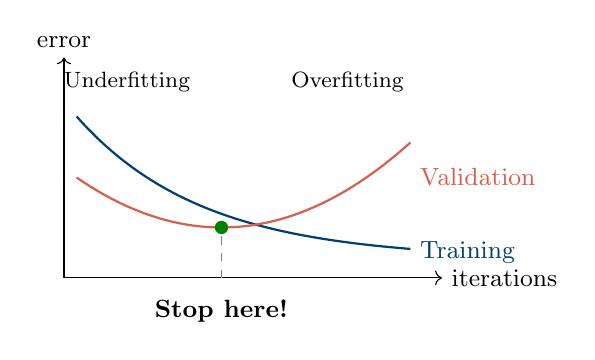
\begin{tikzpicture}[scale=0.8]
    % Axes
    \draw[->] (0, 0) -- (6, 0) node[right] {\small iterations};
    \draw[->] (0, 0) -- (0, 3.5) node[above] {\small error};

    % Training error (decreasing)
    \draw[thick, ThemeBlue, domain=0.2:5.5, samples=50] plot (\x, {2.5*exp(-0.5*\x) + 0.3});
    \node[ThemeBlue, right] at (5.5, 0.4) {\small Training};

    % Validation error (U-shaped)
    \draw[thick, AccentOrange, domain=0.2:5.5, samples=50] plot (\x, {0.15*(\x-2.5)^2 + 0.8});
    \node[AccentOrange, right] at (5.5, 1.6) {\small Validation};

    % Optimal point
    \draw[dashed, gray] (2.5, 0) -- (2.5, 0.8);
    \fill[AccentGreen] (2.5, 0.8) circle (3pt);
    \node[below] at (2.5, -0.2) {\small \textbf{Stop here!}};

    % Annotations
    \node[above, font=\footnotesize] at (1, 2.8) {Underfitting};
    \node[above, font=\footnotesize] at (4.5, 2.8) {Overfitting};
  \end{tikzpicture}
  \end{center}

  \vspace{0.3em}
  \textbf{Early stopping:} Stop training when validation error starts increasing

  \vspace{0.3em}
  In sklearn: \texttt{early\_stopping=True} monitors a validation set and stops automatically.
\end{frame}

%----------------------------------------------------------------------------------------

\begin{frame}{Regularization Strategy 2: Architecture Choices}

  \textbf{Simpler networks = fewer parameters = less overfitting}

  \vspace{1em}
  \textbf{Choices that affect complexity:}
  \begin{itemize}
    \item \textbf{Number of hidden layers:} More layers = more complex
    \item \textbf{Neurons per layer:} More neurons = more parameters
  \end{itemize}

  \vspace{1em}
  \textbf{Rules of thumb for financial applications:}
  \begin{itemize}
    \item Start with 1 hidden layer
    \item Number of neurons: between $p$ (number of features) and $2p$
    \item Add complexity only if validation performance improves
  \end{itemize}

  \vspace{1em}
  \begin{block}{Practical Advice}
    In finance, simpler networks often work as well as complex ones. Don't assume ``deep'' is better --- it rarely is with limited data.
  \end{block}
\end{frame}

%----------------------------------------------------------------------------------------

\begin{frame}{Putting It All Together: Hyperparameters}

  \textbf{Key choices when using neural networks:}

  \vspace{0.5em}
  \begin{center}
  \begin{tabular}{lp{6cm}}
    \toprule
    \textbf{Hyperparameter} & \textbf{Guidance} \\
    \midrule
    Hidden layers & Start with 1, rarely need more than 2 for finance \\
    Neurons per layer & Start with $\sim$50--100, tune via CV \\
    Activation & ReLU for hidden layers; linear/sigmoid for output \\
    Learning rate & Start with default (0.001); Adam adapts it \\
    Regularization ($\alpha$) & Tune via cross-validation (e.g., 0.0001 to 0.1) \\
    Early stopping & Almost always use it \\
    \bottomrule
  \end{tabular}
  \end{center}

  \vspace{1em}
  \textbf{Validation is essential:} Use time-series cross-validation (no shuffling!) to select hyperparameters.
\end{frame}

%----------------------------------------------------------------------------------------

\begin{frame}{Feature Scaling: Critical for Neural Networks}

  \textbf{Unlike trees, neural networks are sensitive to feature scales}

  \vspace{1em}
  \textbf{Why?}
  \begin{itemize}
    \item Gradient descent works better when features are on similar scales
    \item Large-scale features dominate the learning process
    \item Activation functions can saturate with extreme values
  \end{itemize}

  \vspace{1em}
  \textbf{Solution: Standardize your features}
  \[
  x_j^{\text{scaled}} = \frac{x_j - \bar{x}_j}{s_j}
  \]
  where $\bar{x}_j$ is the mean and $s_j$ is the standard deviation

  \vspace{0.5em}
  \begin{block}{Important}
    \begin{itemize}
      \item Compute mean and std on \textbf{training data only}
      \item Apply the same transformation to validation/test data
      \item sklearn's \texttt{StandardScaler} handles this
    \end{itemize}
  \end{block}
\end{frame}

%----------------------------------------------------------------------------------------
\section{Revisiting Market Timing}
%----------------------------------------------------------------------------------------

\begin{frame}{Recap: What We Learned in Part I}

  \textbf{Neural networks: the key ideas}
  \begin{itemize}
    \item Neurons: weighted sum $\rightarrow$ non-linear activation $\rightarrow$ output
    \item Multi-layer perceptrons (MLPs): stack neurons into layers
    \item Learning: gradient descent minimizes a loss function
    \item Regularization: Early stopping, architecture choice
  \end{itemize}

  \vspace{1em}
  \textbf{Key advantages over previous methods:}
  \begin{itemize}
    \item Smooth predictions (unlike trees)
    \item Automatic non-linearities and interactions (unlike linear models)
    \item Universal approximation capability
  \end{itemize}

  \vspace{0.5em}
  \begin{block}{Today's Question}
    Can neural networks improve on Ridge and Random Forest for \highlight{market timing}?
  \end{block}
\end{frame}

%----------------------------------------------------------------------------------------

\begin{frame}{Benchmarks from Previous Weeks}

  \textbf{What we found so far (Weeks 2--3):}

  \vspace{0.5em}
  \begin{center}
  \begin{tabular}{lcc}
    \toprule
    \textbf{Method} & \textbf{Sharpe Ratio} & \textbf{Ann.\ Return (\%)} \\
    \midrule
    Buy \& Hold & 0.46 & 6.9 \\
    Ridge & 0.64 & 10.3 \\
    Random Forest & 0.47 & 7.0 \\
    \bottomrule
  \end{tabular}
  \end{center}

  \vspace{1em}
  \textbf{Key findings:}
  \begin{itemize}
    \item Market timing is \highlight{very hard}
    \item Ridge provides meaningful improvement over buy-and-hold
    \item Random Forest only marginally better than passive
    \item Statistical accuracy $\neq$ economic performance
  \end{itemize}

  \vspace{0.5em}
  \textbf{Today's question:} Can neural networks do better?
\end{frame}

%----------------------------------------------------------------------------------------

\begin{frame}{The Promise of Neural Networks}

  \textbf{Potential advantages:}
  \begin{enumerate}
    \item \highlight{Smooth non-linearity:} Unlike trees, MLPs produce smooth functions
    \item \highlight{Flexible interactions:} Network learns which combinations matter
    \item \highlight{Universal approximation:} Can represent any continuous function
  \end{enumerate}

  \vspace{1em}
  \textbf{Potential disadvantages:}
  \begin{itemize}
    \item Many parameters $\rightarrow$ overfitting risk
    \item Requires careful tuning (architecture, regularization)
    \item Computationally more expensive
    \item Black box: hard to interpret
  \end{itemize}

  \vspace{0.5em}
  \textbf{Empirical question:} Do the advantages outweigh the disadvantages for market timing with limited data?
\end{frame}

%----------------------------------------------------------------------------------------
\section{Out-of-Sample Performance}
%----------------------------------------------------------------------------------------

\begin{frame}{Implementation: Methods Compared}

  \textbf{Linear methods (from Week 2):}
  \begin{itemize}
    \item Ridge, Lasso, Elastic Net
  \end{itemize}

  \vspace{0.3em}
  \textbf{Tree-based methods (from Week 3):}
  \begin{itemize}
    \item Random Forest, Gradient Boosting (XGBoost)
  \end{itemize}

  \vspace{0.3em}
  \textbf{Neural network (new):}
  \begin{itemize}
    \item MLPRegressor with one hidden layer
  \end{itemize}

  \vspace{1em}
  \textbf{Common setup:}
  \begin{itemize}
    \item Data: GWZ (2024) --- 25 predictors, monthly 1956--2021
    \item Walk-forward prediction (expanding window)
    \item Initial training: 120 months
    \item Hyperparameters: Time-series cross-validation
  \end{itemize}
\end{frame}

%----------------------------------------------------------------------------------------

\begin{frame}{From Predictions to Portfolios}

  \textbf{Recall from Weeks 2--3:} Mean-variance timing weights
  \[
  \omega_t = \frac{1}{\gamma} \cdot \frac{\widehat{r}_{t+1}}{\widehat{\sigma}^2_t}
  \]

  \vspace{0.3em}
  \begin{itemize}
    \item $\widehat{r}_{t+1}$: Predicted excess return (from each model)
    \item $\widehat{\sigma}^2_t$: Rolling variance estimate (60-month window)
    \item $\gamma = 5$: Risk aversion
    \item Weights constrained to $[-0.5, 1.5]$
  \end{itemize}

  \vspace{1em}
  \textbf{Portfolio return:}
  \[
  r^{portfolio}_{t+1} = \omega_t \cdot r^{market}_{t+1} +(1-\omega_t)\cdot r_t^f
  \]

  \vspace{0.5em}
  \textbf{Benchmark:} Buy-and-hold ($\omega_t = 1$ always)
\end{frame}

%----------------------------------------------------------------------------------------

\begin{frame}{The Main Result: MLP Dominates Economically}

  \begin{center}
  \resizebox{1\textwidth}{!}{\begin{tabular}{lccc}
    \toprule
    \textbf{Method} & \textbf{$R^2_{OS}$ (\%)}  & \textbf{Sharpe Ratio} & \textbf{Ann.\ Return (\%)}\\
    \midrule
    Buy \& Hold & --- & 0.46 & 6.86 \\
    \midrule
    OLS & $-13.85$ & 0.65 & 10.50 \\
    Ridge & $-11.94$ & 0.64 & 10.33 \\
    Lasso & $-0.03$ & 0.41 & 4.81 \\
    Elastic Net & $+1.02$ & 0.53 & 6.08 \\
    \midrule
    Random Forest & $-0.75$ & 0.47 & 6.97 \\
    \midrule
    \highlight{MLP} & \highlight{$-0.68$} & \highlight{0.74} & \highlight{11.48} \\
    \bottomrule
  \end{tabular}}
  \end{center}

  \vspace{0.5em}
  \textbf{Key puzzle:} MLP has \highlight{slight negative $R^2_{OS}$} but achieves the \highlight{highest Sharpe ratio}!

  \vspace{0.3em}
  \textit{Statistical accuracy $\neq$ Economic value}
\end{frame}

%----------------------------------------------------------------------------------------

\begin{frame}{Cumulative Wealth (Gross)}

  \begin{center}
  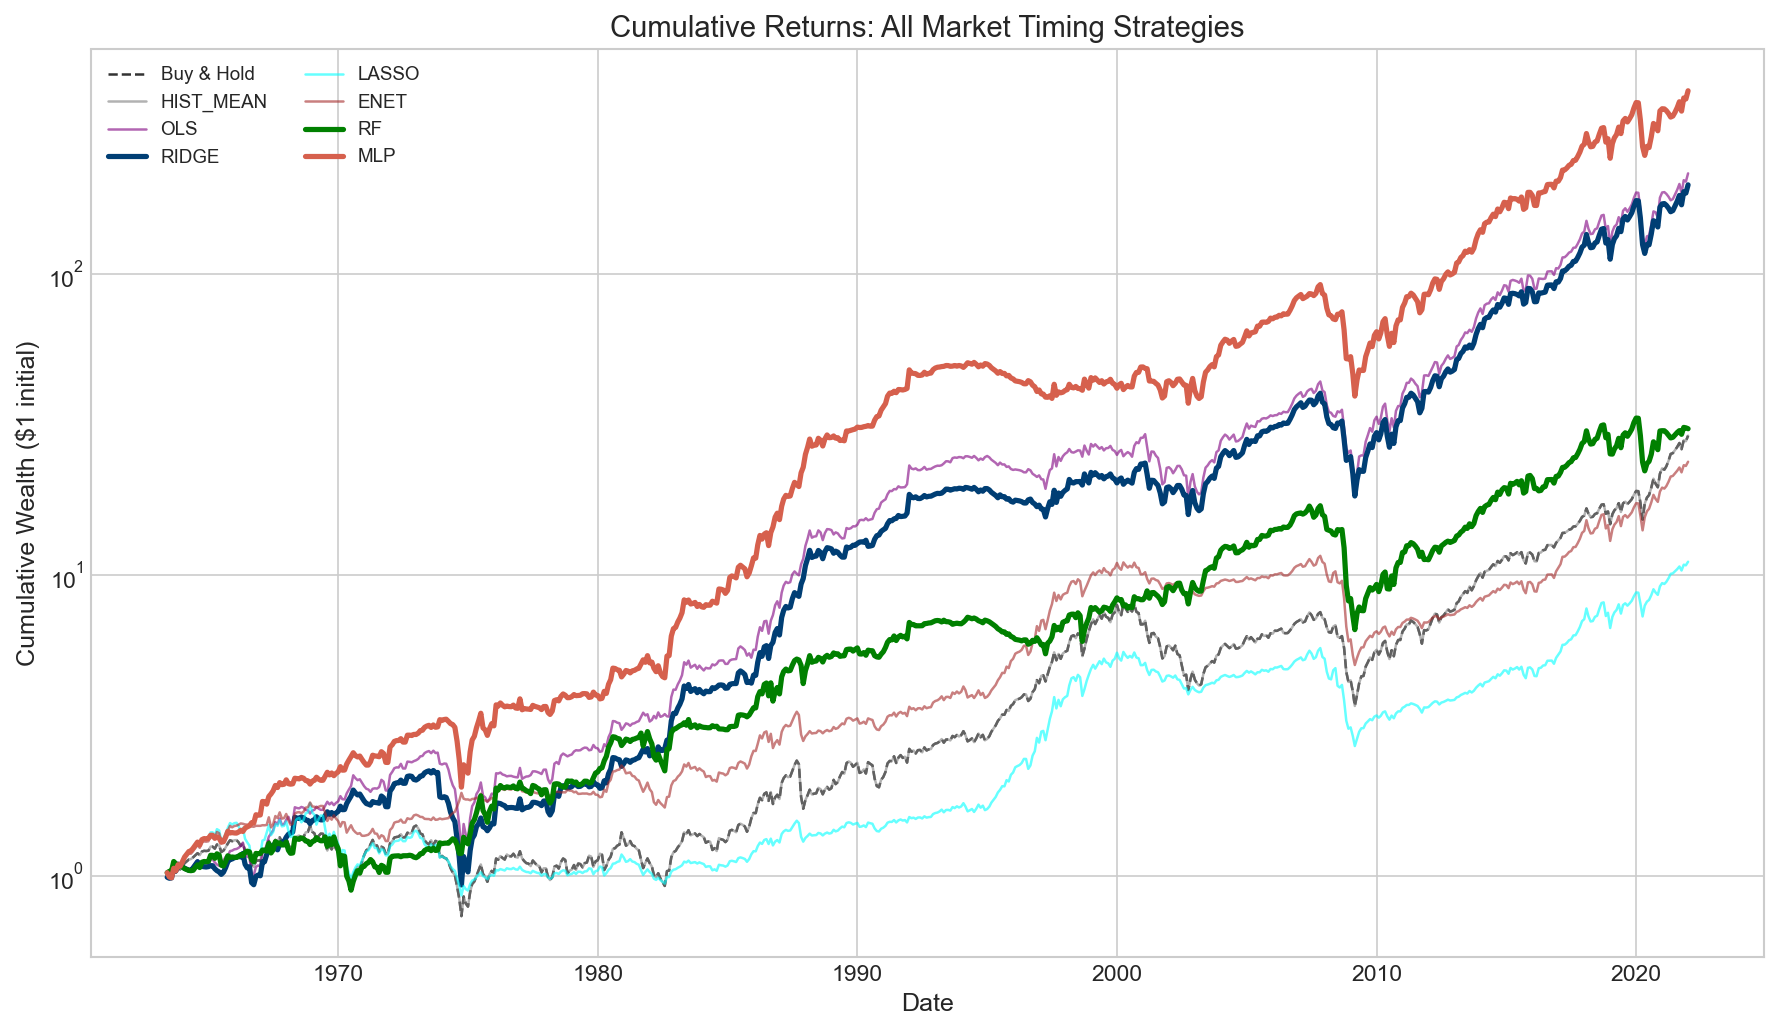
\includegraphics[width=0.95\textwidth]{Figures/fig_cumulative_returns_all.png}
  \end{center}

  \vspace{0.3em}
  \textit{Cumulative wealth from \$1 initial investment. Log scale. MLP (red) clearly dominates throughout the sample.}
\end{frame}

%----------------------------------------------------------------------------------------

\begin{frame}{The $R^2_{OS}$ vs.\ Sharpe Ratio Puzzle}

  \textbf{How can MLP have negative $R^2_{OS}$ but the best Sharpe ratio?}

  \vspace{1em}
  \begin{enumerate}
    \item \textbf{$R^2_{OS}$ measures average squared error}
    \begin{itemize}
      \item Penalizes large errors heavily (squared!)
      \item A few big mistakes hurt $R^2$ a lot
    \end{itemize}

    \vspace{0.5em}
    \item \textbf{Sharpe ratio depends on \highlight{when} you're right}
    \begin{itemize}
      \item Being right when it matters most (big moves) is valuable
      \item Small errors when market is flat don't hurt much
    \end{itemize}

    \vspace{0.5em}
    \item \textbf{Direction matters more than magnitude}
    \begin{itemize}
      \item Predicting $+1\%$ when actual is $+5\%$ still makes money
      \item Getting the \highlight{sign right} is what counts for portfolios
    \end{itemize}
  \end{enumerate}

  \vspace{0.5em}
  \begin{block}{Lesson}
    Always evaluate models on their \highlight{intended use case}. For trading, economic metrics matter more than $R^2$.
  \end{block}
\end{frame}

%----------------------------------------------------------------------------------------

\begin{frame}{Interpreting the Results}

  \textbf{Key observations:}
  \begin{enumerate}
    \item MLP achieves the \highlight{best performance} across all metrics
    \begin{itemize}
      \item Highest Sharpe ratio (0.74)
      \item Highest total return (40,381\%)
      \item Consistent outperformance throughout the sample
    \end{itemize}

    \vspace{0.5em}
    \item Ridge is a strong second
    \begin{itemize}
      \item Sharpe of 0.64 --- still excellent
      \item Much simpler to implement and tune
    \end{itemize}

    \vspace{0.5em}
    \item Random Forest disappoints
    \begin{itemize}
      \item Sharpe of 0.47 --- barely beats buy-and-hold
      \item Trees' piecewise-constant predictions may not suit this problem
    \end{itemize}

    \vspace{0.5em}
    \item Lasso underperforms
    \begin{itemize}
      \item Too aggressive variable selection?
    \end{itemize}
  \end{enumerate}
\end{frame}

%----------------------------------------------------------------------------------------

\begin{frame}{Turnover Analysis}

  \textbf{Average monthly weight change (\%):}

  \vspace{0.5em}
  \begin{center}
  \begin{tabular}{lc}
    \toprule
    \textbf{Strategy} & \textbf{Avg.\ Turnover (\%/month)} \\
    \midrule
    Buy \& Hold & 0.0 \\
    Historical Mean & 0.0 \\
    \midrule
    Lasso & 1.8 \\
    Elastic Net & 11.6 \\
    Random Forest & 37.8 \\
    \midrule
    \highlight{MLP} & \highlight{40.1} \\
    Ridge & 46.6 \\
    OLS & 46.6 \\
    \bottomrule
  \end{tabular}
  \end{center}

  \vspace{0.5em}
  \textbf{Key observation:} MLP has \highlight{lower turnover} than OLS/Ridge
  \begin{itemize}
    \item Smooth predictions $\rightarrow$ gradual weight adjustments
    \item Less sensitive to transaction costs than linear methods
  \end{itemize}
\end{frame}

%----------------------------------------------------------------------------------------

\begin{frame}{Robustness: After Transaction Costs (50 bps)}

  \begin{center}
  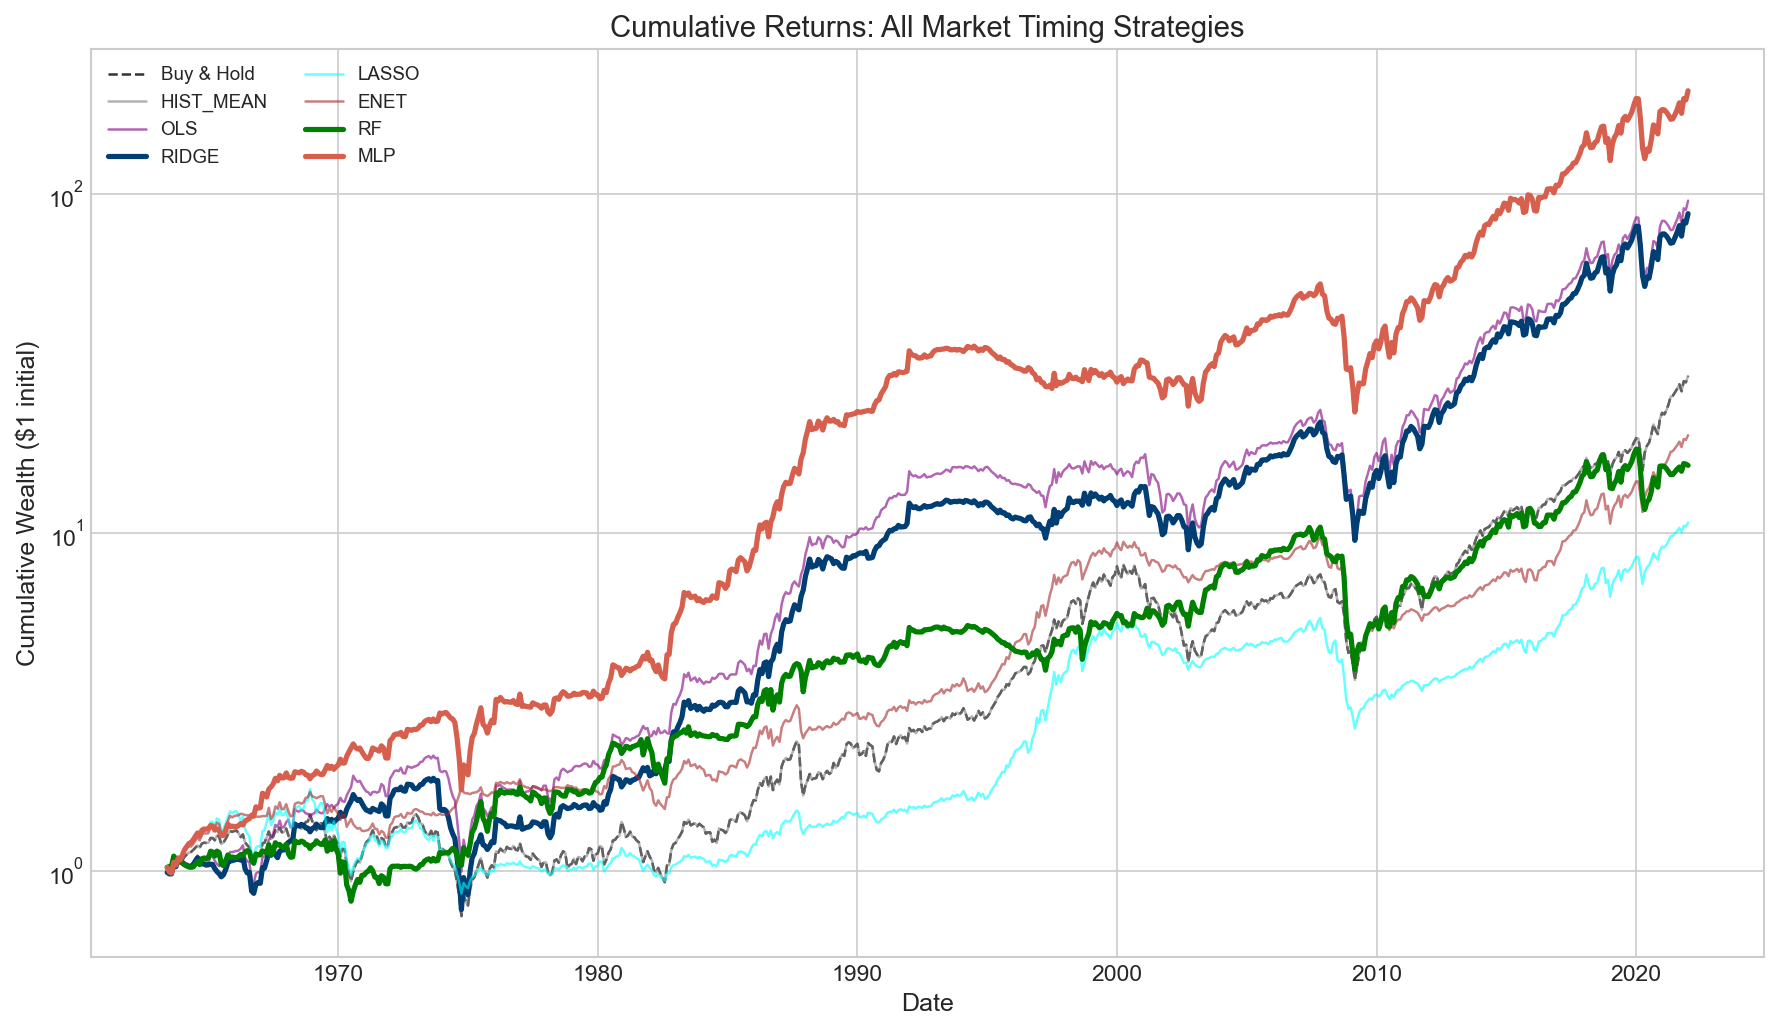
\includegraphics[width=0.95\textwidth]{Figures/fig_cumulative_returns_all_net.png}
  \end{center}

  \vspace{0.3em}
  \textit{Net of 50 bps transaction costs per rebalancing. MLP remains dominant.}
\end{frame}

%----------------------------------------------------------------------------------------

\begin{frame}{Performance After Transaction Costs}

  \begin{center}
  \resizebox{1\textwidth}{!}{\begin{tabular}{lcccc}
    \toprule
    \textbf{Strategy} & \textbf{Turnover} & \textbf{Sharpe (Gross)} & \textbf{Sharpe (Net)} & \textbf{$\Delta$} \\
    \midrule
    Buy \& Hold & 0.0 & 0.46 & 0.46 & 0.00 \\
    \midrule
    Lasso & 1.8 & 0.41 & 0.40 & $-0.01$ \\
    Elastic Net & 11.6 & 0.53 & 0.50 & $-0.03$ \\
    Random Forest & 37.8 & 0.47 & \textcolor{AccentOrange}{0.39} & $-0.08$ \\
    \midrule
    \highlight{MLP} & 40.1 & \highlight{0.74} & \highlight{0.66} & $-0.08$ \\
    Ridge & 46.6 & 0.64 & 0.56 & $-0.08$ \\
    OLS & 46.6 & 0.65 & 0.56 & $-0.09$ \\
    \bottomrule
  \end{tabular}}
  \end{center}

  \vspace{0.5em}
  \textbf{Observations:}
  \begin{itemize}
    \item MLP remains best even after 50 bps costs (Sharpe: 0.66)
    \item Higher turnover $\rightarrow$ larger Sharpe degradation
    \item Random Forest falls \textit{below} buy-and-hold after costs!
  \end{itemize}
\end{frame}

%----------------------------------------------------------------------------------------

\begin{frame}{Why Does MLP Outperform?}

  \textbf{Potential explanations:}

  \vspace{0.5em}
  \begin{enumerate}
    \item \textbf{Smooth non-linearity:}
    \begin{itemize}
      \item MLP captures non-linear relationships smoothly
      \item Trees produce ``blocky'' predictions $\rightarrow$ higher turnover
    \end{itemize}

    \vspace{0.5em}
    \item \textbf{Flexible interactions:}
    \begin{itemize}
      \item Network learns which predictor combinations matter
      \item More efficient than manual specification
    \end{itemize}

    \vspace{0.5em}
    \item \textbf{Regularization works well:}
    \begin{itemize}
      \item L2 penalty + early stopping prevents overfitting
      \item Similar principle to why Ridge beats OLS
    \end{itemize}

    \vspace{0.5em}
    \item \textbf{Lower turnover:}
    \begin{itemize}
      \item Smooth predictions $\rightarrow$ gradual weight changes
      \item Robust to transaction costs
    \end{itemize}
  \end{enumerate}
\end{frame}

%----------------------------------------------------------------------------------------

\begin{frame}{A Caveat: Maximum Drawdowns}

  \textbf{All timing strategies have significant drawdowns:}

  \vspace{0.5em}
  \begin{center}
  \begin{tabular}{lc}
    \toprule
    \textbf{Strategy} & \textbf{Max Drawdown (\%)} \\
    \midrule
    Buy \& Hold & $-54.3$ \\
    \midrule
    Lasso & $-52.7$ \\
    Elastic Net & $-56.6$ \\
    OLS & $-56.4$ \\
    MLP & $-57.4$ \\
    Ridge & $-58.3$ \\
    Random Forest & $-61.2$ \\
    \bottomrule
  \end{tabular}
  \end{center}

  \vspace{0.5em}
  \textbf{Key point:} Higher returns come with similar or \textit{higher} drawdowns
  \begin{itemize}
    \item Timing strategies lever up in good times
    \item When wrong, losses are magnified
    \item Real-world implementation requires risk management
  \end{itemize}
\end{frame}

%----------------------------------------------------------------------------------------
\section{Neural Networks for Classification}
%----------------------------------------------------------------------------------------

\begin{frame}{MLPClassifier: Credit Risk Application}

  \textbf{Same architecture, different output:}

  \vspace{0.5em}
  \begin{center}
  \begin{tabular}{lcc}
    \toprule
    & \textbf{MLPRegressor} & \textbf{MLPClassifier} \\
    \midrule
    Output layer activation & Linear (identity) & Sigmoid / Softmax \\
    Loss function & MSE & Cross-entropy \\
    Output & Predicted value & Probability \\
    \bottomrule
  \end{tabular}
  \end{center}

  \vspace{1em}
  \textbf{sklearn interface is nearly identical:}
  \begin{itemize}
    \item Same \texttt{hidden\_layer\_sizes}, \texttt{alpha}, \texttt{solver}
    \item Use \texttt{predict\_proba()} to get probabilities
    \item \texttt{class\_weight} \highlight{not available} --- unlike Random Forest / Logistic
  \end{itemize}
\end{frame}

%----------------------------------------------------------------------------------------

\begin{frame}{Handling Class Imbalance with MLPClassifier}

  \textbf{Problem:} \texttt{MLPClassifier} doesn't have \texttt{class\_weight} parameter

  \vspace{1em}
  \textbf{Solutions:}
  \begin{enumerate}
    \item \textbf{Resampling:}
    \begin{itemize}
      \item Oversample minority class (SMOTE)
      \item Undersample majority class
      \item Use \texttt{imbalanced-learn} library
    \end{itemize}

    \vspace{0.5em}
    \item \textbf{Threshold tuning:}
    \begin{itemize}
      \item Train with default threshold (0.5)
      \item Adjust classification threshold based on cost trade-offs
      \item Choose threshold that maximizes F1 or business objective
    \end{itemize}

    \vspace{0.5em}
    \item \textbf{Custom loss:} More advanced --- requires leaving sklearn
  \end{enumerate}

  \vspace{0.5em}
  \textit{For your projects: threshold tuning is often the simplest effective approach.}
\end{frame}

%----------------------------------------------------------------------------------------

\begin{frame}{Expected Results for Credit Risk}

  \textbf{Based on the literature and typical findings:}

  \vspace{0.5em}
  \begin{center}
  \begin{tabular}{lc}
    \toprule
    \textbf{Method} & \textbf{AUC (typical range)} \\
    \midrule
    Logistic Regression & 0.70--0.75 \\
    Random Forest & 0.72--0.77 \\
    XGBoost & 0.73--0.78 \\
    MLP & 0.72--0.77 \\
    \bottomrule
  \end{tabular}
  \end{center}

  \vspace{1em}
  \textbf{Key points:}
  \begin{itemize}
    \item MLPClassifier typically \highlight{competitive but not dominant}
    \item With large datasets (millions of loans), MLPs can match boosting
    \item Interpretability remains a challenge for regulatory applications
    \item Probability calibration often needed (use \texttt{CalibratedClassifierCV})
  \end{itemize}
\end{frame}

%----------------------------------------------------------------------------------------
\section{When Do Neural Networks Help?}
%----------------------------------------------------------------------------------------

\begin{frame}{Evidence from the Finance Literature}

  \textbf{Gu, Kelly \& Xiu (2020, \textit{RFS}):}
  \begin{itemize}
    \item Compared many ML methods for stock return prediction
    \item Neural networks: competitive but not always best
    \item Gains most pronounced with \highlight{many features} and \highlight{large samples}
  \end{itemize}

  \vspace{0.5em}
  \textbf{Chen, Pelger \& Zhu (2024, \textit{Management Science}):}
  \begin{itemize}
    \item Deep learning for asset pricing
    \item Benefits emerge with \highlight{cross-sectional data} (many stocks)
    \item Time-series prediction (market timing): modest improvements
  \end{itemize}

  \vspace{0.5em}
  \textbf{Goyal, Welch \& Zafirov (2024, \textit{RFS}):}
  \begin{itemize}
    \item Comprehensive comparison for equity premium prediction
    \item ``No method consistently dominates''
    \item Simple methods often as good as complex ones
  \end{itemize}
\end{frame}

%----------------------------------------------------------------------------------------

\begin{frame}{Conditions Favoring Neural Networks}

  \textbf{Our results suggest MLPs help when:}
  \begin{itemize}
    \item \textcolor{AccentGreen}{\checkmark} Relationships are \highlight{non-linear but smooth}
    \item \textcolor{AccentGreen}{\checkmark} Interactions between predictors matter
    \item \textcolor{AccentGreen}{\checkmark} Regularization is applied carefully
    \item \textcolor{AccentGreen}{\checkmark} Turnover costs are a concern (smooth predictions help)
  \end{itemize}

  \vspace{1em}
  \textbf{Simpler methods may suffice when:}
  \begin{itemize}
    \item \textcolor{AccentOrange}{$\times$} Interpretability is required (regulatory, audit)
    \item \textcolor{AccentOrange}{$\times$} Computational resources are very limited
    \item \textcolor{AccentOrange}{$\times$} Quick iteration/debugging is needed
  \end{itemize}

  \vspace{0.5em}
  \begin{block}{Revised View}
    With proper regularization, MLPs \textit{can} outperform in financial time-series --- but the gains depend on careful implementation.
  \end{block}
\end{frame}

%----------------------------------------------------------------------------------------

\begin{frame}{Computational Considerations}

  \textbf{Neural networks are more expensive:}

  \vspace{0.5em}
  \begin{center}
  \begin{tabular}{lcc}
    \toprule
    \textbf{Method} & \textbf{Training Time} & \textbf{Tuning Complexity} \\
    \midrule
    Ridge & Very fast & 1 hyperparameter \\
    Random Forest & Moderate & 2--3 hyperparameters \\
    XGBoost & Moderate & 4--5 hyperparameters \\
    MLP & Slower & 3--5 hyperparameters \\
    \bottomrule
  \end{tabular}
  \end{center}

  \vspace{1em}
  \textbf{Practical implications:}
  \begin{itemize}
    \item Walk-forward with frequent refitting can be slow
    \item Hyperparameter search is more expensive (architecture choices)
    \item For production: consider computational budget
  \end{itemize}

  \vspace{0.5em}
  \textit{In our GWZ application: MLP takes 5--10$\times$ longer than Ridge to tune and fit.}
\end{frame}

%----------------------------------------------------------------------------------------

\begin{frame}{Caveats and Considerations}

  \textbf{Before concluding ``MLPs always win'':}

  \vspace{0.5em}
  \begin{enumerate}
    \item \textbf{In-sample optimization:}
    \begin{itemize}
      \item Results may partly reflect lucky hyperparameter choices
      \item Different random seeds can give different results
    \end{itemize}

    \vspace{0.3em}
    \item \textbf{Structural breaks:}
    \begin{itemize}
      \item Patterns learned in 1960s--1990s may not persist
      \item MLP's flexibility could adapt or could overfit
    \end{itemize}

    \vspace{0.3em}
    \item \textbf{Implementation risk:}
    \begin{itemize}
      \item More moving parts = more things that can go wrong
      \item Ridge is harder to ``break''
    \end{itemize}

    \vspace{0.3em}
    \item \textbf{Interpretability:}
    \begin{itemize}
      \item ``Why is the model bullish today?''
      \item Regulators and risk managers need answers
    \end{itemize}
  \end{enumerate}

  \vspace{0.5em}
  \textit{Strong results deserve scrutiny --- especially in finance!}
\end{frame}

%----------------------------------------------------------------------------------------
\section{Summary and Next Steps}
%----------------------------------------------------------------------------------------

\begin{frame}{Key Takeaways from Today}

  \begin{enumerate}
    \item \textbf{MLP achieves the best performance for market timing}
    \begin{itemize}
      \item Sharpe of 0.74 (gross), 0.66 (net) vs.\ 0.46 for buy-and-hold
      \item Terminal wealth 14$\times$ higher than passive investing
    \end{itemize}

    \vspace{0.3em}
    \item \textbf{Smooth non-linearity matters}
    \begin{itemize}
      \item MLP captures non-linear patterns with low turnover
      \item Trees' piecewise-constant predictions create high turnover
    \end{itemize}

    \vspace{0.3em}
    \item \textbf{Regularization is essential}
    \begin{itemize}
      \item Simple architecture + early stopping prevents overfitting
      \item \highlight{Always scale features} with StandardScaler
    \end{itemize}

    \vspace{0.3em}
    \item \textbf{Results are robust to transaction costs}
    \begin{itemize}
      \item MLP remains best after 50 bps costs
      \item Random Forest hurt most by turnover
    \end{itemize}
  \end{enumerate}
\end{frame}

%----------------------------------------------------------------------------------------

\begin{frame}{Readings}

  \textbf{Readings:}
  \begin{itemize}
    \item James et al.\ (2023), \textit{ISLP}, Chapter 10 \hfill \textit{[Recomm.]}
    \item Gu, Kelly \& Xiu (2020), ``Empirical Asset Pricing via Machine Learning,'' \textit{Review of Financial Studies} \hfill \textit{[Supp.]}
    \item Chen, Pelger \& Zhu (2024), ``Deep Learning in Asset Pricing'', Management Science \hfill \textit{[Supp.]}
  \end{itemize}


\end{frame}

%----------------------------------------------------------------------------------------

\begin{frame}[plain]
  \centering
  \vfill
  {\Large Questions?}
  \vfill
\end{frame}

\end{document}
